\documentclass[a4paper]{article}   
\usepackage{pgfplots}  
\usepackage{scalefnt} % 文本大小放缩宏包
        
\begin{document}
{% 调整字体大小
\scalefont{1.2}
    % 罗尔定理                    
    \begin{tikzpicture}[line width=1.2pt]      
        % 画坐标系
        \draw[->] (-1.2,0) -- (8.2,0) node[right] {$x$};
        \draw[->] (0,-1.2) -- (0,5) node[above] {$y$};
        \draw (0, 0) node[below left] {O};
        
        % sin
        \draw[domain=1:7.28] plot (\x, {2 + sin((\x - 1.5236) r)});
        \draw (4.7, 2.5) node[right] {$f$};
        
        % 切线
        \draw (2.07, 3) -- (4.07, 3);
        
        % 辅助线及各种记号
        \draw[dashed, color=red] (1, 1.5) -- (7.28, 1.5);
        \draw[dashed] (3.09, 3) -- (3.09, 0) node[below] {$\xi$};
        \draw[dashed] (1, 1.5) -- (1, 0) node[below] {$a$};
        \draw[dashed] (7.28, 1.5) -- (7.28, 0) node[below] {$b$};
        \draw[dashed] (1, 1.5) -- (0, 1.5) node[left] {$f(a) = f(b)$};
    \end{tikzpicture}  
    
    % 拉格朗日中值定理
    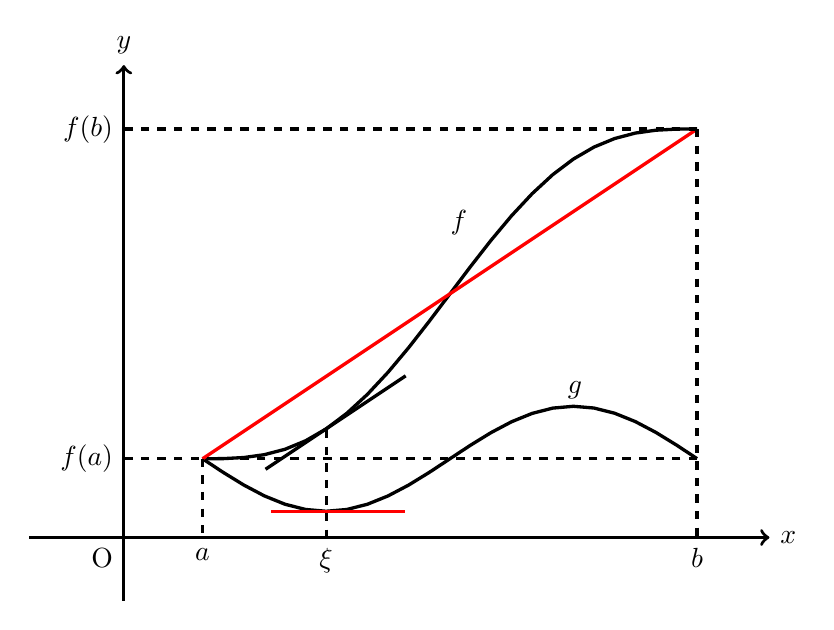
\begin{tikzpicture}[line width=1.2pt]        
        % 画坐标系
        \draw[->] (-1.2,0) -- (8.2,0) node[right] {$x$};
        \draw[->] (0,-1.2/1.5) -- (0,9/1.5) node[above] {$y$};
        \draw (0, 0) node[below left] {O};
        
        % f = x + sin
        \draw[domain=1:7.28] plot (\x, {(1.5 - sin((\x - 1) r) + (\x - 1))/1.5});
        \draw (4.5, 6/1.5) node[left] {$f$};
        
        % g = sin
        \draw[domain=1:7.28] plot (\x, {(1.5 - sin((\x - 1) r))/1.5});
        \draw (5.5, 2.8/1.5) node[right] {$g$};
        
        % 切线
        \draw[color=red] (1.87, 0.5/1.5) -- (3.57, 0.5/1.5);
        \draw[domain=1.8:3.58] plot (\x, {(\x - 0.5)/1.5});
        
        % 辅助线及各种记号
        \draw[color=red] (1, 1.5/1.5) -- (7.28, 7.78/1.5);
        \draw[dashed] (2.57, 2.047/1.5) -- (2.57, 0) node[below] {$\xi$};
        \draw[dashed] (7.28, 7.78/1.5) -- (7.28, 0) node[below] {$b$};
        \draw[dashed] (7.28, 7.78/1.5) -- (0, 7.78/1.5) node[left] {$f(b)$};
        \draw[dashed] (1, 1.5/1.5) -- (1, 0) node[below] {$a$};
        \draw[dashed] (7.28, 1.5/1.5) -- (0, 1.5/1.5) node[left] {$f(a)$};
    \end{tikzpicture} 
    
    \begin{tikzpicture}[line width=1.2pt]          
        % 画坐标系
        \draw[->] (-5,0) -- (5,0) node[right] {$x$};
        \draw[->] (0,-4) -- (0,4) node[above] {$y$};
        \draw (0, 0) node[below left] {O};
        
        % f = 1
        \draw[domain=0:4] plot (\x, 2);
        \draw[fill=white] (0,2) circle (3pt);
        % f = -1
        \draw[domain=-4:0] plot (\x, -2);
        
        % 辅助线及各种记号
        \draw[dashed] (4, 2) -- (4, 0) node[below] {$1$};
        \draw[dashed] (-4, -2) -- (-4, 0) node[above] {$-1$};
    \end{tikzpicture} 
    
    % 零点存在定理
    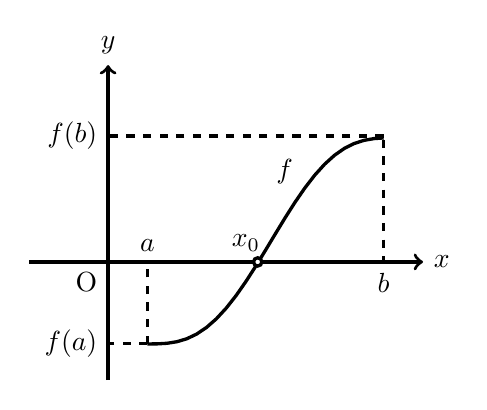
\begin{tikzpicture}[line width=1.2pt, scale = 0.5]          
        % 画坐标系
        \draw[->] (-2,0) -- (8,0) node[right] {$x$};
        \draw[->] (0,-3) -- (0,5) node[above] {$y$};
        \draw (0, 0) node[below left] {O};
        
        % f = sin x
        \draw[domain=1:7] plot (\x, {(-2.5- sin((\x - 1) r) + (\x - 1))/1.2});
        
        % 辅助线及各种记号
        \draw[dashed] (1, -2.08) -- (1, 0) node[above] {$a$};
        \draw[dashed] (1, -2.08) -- (0, -2.08) node[left] {$f(a)$};
        \draw[dashed] (7, 3.1) -- (7, 0) node[below] {$b$};
        \draw[dashed] (7, 3.2) -- (0, 3.2) node[left] {$f(b)$};
        \draw (4, 2.3) node[right] {$f$};
        
        \draw[fill=white] (3.8,0) circle (3pt);
        \draw (3.5, 0) node[above] {$x_0$};
    \end{tikzpicture} 
}          
\end{document}    
